\documentclass[parskip=half]{scrartcl}

%\usepackage{fontspec, unicode-math}
%\setmainfont{Libertinus Serif}
%\setsansfont{Libertinus Sans}
%\setmathfont{Libertinus Math}

\usepackage{tikz}

\usetikzlibrary{
    fit,
    spy,
    backgrounds,
    svg.path,
    arrows,
    arrows.meta,
    positioning,
    calc,
    patterns,
    external,
    decorations,
    decorations.markings,
    decorations.shapes,
}

\tikzset {
    line/.style={semithick},
    tip/.style args = {#1 and #2}{
        line,
        ->,
        >=stealth,
        shorten >= #1,
        shorten <= #2
    },
    tip/.default = {0pt and 0pt},
    bitip/.style args = {#1 and #2}{
        line,
        <->,
        >=stealth,
        shorten >= #1,
        shorten <= #2
    },
    bitip/.default = {0pt and 0pt},
    rtip/.style = {
        line,
        <-,
        >=stealth
    },
    vtip/.style = {
        line,
        <-,
        >=stealth,
        shorten >=2pt, 
        shorten <=2pt
    },
    dot diameter/.store in = \dotdiameter,
    dot diameter = 1.25pt,
    dot spacing/.store in = \dotspacing,
    dot spacing = 1.3pt,
    dots/.style = {
        line width = \dotdiameter,
        line cap = round,
        dash pattern = on 0pt off \dotspacing
    },
    every pin/.style = {pin edge = {rtip, black}, fill = white, inner sep = 1pt},
    dotgrid/.style={line width = #1, dash pattern = on 0pt off 1.2pt, line cap = round},
    dotgrid/.default=0.8pt
}

%% fix pin and label anchors and placement
%% taken from https://tex.stackexchange.com/questions/246995/tikz-adjusting-pin-anchor
%\makeatletter
%\newcommand*\ifStrInTF[2]{%
%  \edef\tikz@temp{{#1}{#2}}%
%  \expandafter\pgfutil@in@\tikz@temp
%  \ifpgfutil@in@\expandafter\pgfutil@firstoftwo\else\expandafter\pgfutil@secondoftwo\fi}
%\newcommand*\ifStrEmptyTF[1]{%
%  \def\tikz@temp{#1}\ifx\tikz@temp\pgfutil@empty
%    \expandafter\pgfutil@firstoftwo\else\expandafter\pgfutil@secondoftwo\fi}
%
%\def\tikz@swapanchor#1.#2\tikz@stop#3#4{#1#4#3}
%\newcommand*\tikzAddAnchor[2]{%
%  \ifStrInTF{.}{#1}{%
%    \ifStrEmptyTF{#2}
%      {\edef#1{\expandafter\tikz@swapanchor#1\tikz@stop{}{}}}
%      {\edef#1{\expandafter\tikz@swapanchor#1\tikz@stop{#2}{.}}}%
%  }{%
%    \ifStrEmptyTF{#2}{}% no true
%      {\edef#1{#1.#2}}%
%  }}
%\tikzset{
%  pin anchor/.style={tikz@pin@post/.append style={anchor=#1}},
%  label anchor/.style={tikz@label@post/.append style={anchor=#1}},
%  pin edge pin anchor/.style={
%    append after command={\pgfextra\tikzAddAnchor{\tikzlastnode}{#1}\endpgfextra}%
%  },
%  pin edge parent anchor/.style={
%    append after command={\pgfextra\tikzAddAnchor{\tikz@save@last@node}{#1}\endpgfextra}%
%  }
%}
%\makeatother

% custom drawing commands
\def\showboundingbox{\path[fill=blue, opacity = 0.1] (current bounding box.north west) rectangle (current bounding box.south east);}

% orcid logo, taken from https://tex.stackexchange.com/questions/445563/ieeetran-how-to-include-orcid-in-tex-pdf-with-pdflatex/445583#445583
\definecolor{orcidlogocol}{HTML}{A6CE39}
\tikzset{
    orcidlogo/.pic={
        \fill[orcidlogocol] svg{M256,128c0,70.7-57.3,128-128,128C57.3,256,0,198.7,0,128C0,57.3,57.3,0,128,0C198.7,0,256,57.3,256,128z};
        \fill[white] svg{M86.3,186.2H70.9V79.1h15.4v48.4V186.2z}
                     svg{M108.9,79.1h41.6c39.6,0,57,28.3,57,53.6c0,27.5-21.5,53.6-56.8,53.6h-41.8V79.1z M124.3,172.4h24.5c34.9,0,42.9-26.5,42.9-39.7c0-21.5-13.7-39.7-43.7-39.7h-23.7V172.4z}
                     svg{M88.7,56.8c0,5.5-4.5,10.1-10.1,10.1c-5.6,0-10.1-4.6-10.1-10.1c0-5.6,4.5-10.1,10.1-10.1C84.2,46.7,88.7,51.3,88.7,56.8z};
    },
    orcidlogoblack/.pic={
        \fill[black] svg{M 256 128 c 0 70.7 -57.3 128 -128 128 C 57.3 256 0 198.7 0 128 C 0 57.3 57.3 0 128 0 C 198.7 0 256 57.3 256 128 z};
        \fill[white] svg{M86.3,186.2H70.9V79.1h15.4v48.4V186.2z}
                     svg{M108.9,79.1h41.6c39.6,0,57,28.3,57,53.6c0,27.5-21.5,53.6-56.8,53.6h-41.8V79.1z M124.3,172.4h24.5c34.9,0,42.9-26.5,42.9-39.7c0-21.5-13.7-39.7-43.7-39.7h-23.7V172.4z}
                     svg{M88.7,56.8c0,5.5-4.5,10.1-10.1,10.1c-5.6,0-10.1-4.6-10.1-10.1c0-5.6,4.5-10.1,10.1-10.1C84.2,46.7,88.7,51.3,88.7,56.8z};
    }
}
\def\orcidsymbol{\tikzexternaldisable 
\begin{tikzpicture}[yscale = -1, scale = 0.035, transform shape, baseline = -7.5pt] \pic{orcidlogo}; \end{tikzpicture}}
\def\orcidsymbolblack{\tikzexternaldisable 
\begin{tikzpicture}[yscale = -1, scale = 0.035, transform shape, baseline = -7.5pt] \pic{orcidlogoblack}; \end{tikzpicture}}
\def\orcid#1{\tikzexternaldisable 
\begin{tikzpicture}[yscale = -1, scale = 0.035, transform shape, baseline = -7.5pt] \pic{orcidlogo}; \end{tikzpicture} \textrm{https://orcid.org/#1}}
\def\orcidblack#1{\tikzexternaldisable 
\begin{tikzpicture}[yscale = -1, scale = 0.035, transform shape, baseline = -7.5pt] \pic{orcidlogoblack}; \end{tikzpicture} \textrm{https://orcid.org/#1}}

\newif\ifcircuitsflip

\makeatletter

% drawing styles
\tikzset{
    circuits/general/.style = {thick},
    wire/.style={circuits/general},
    cable/.style={circuits/general, cap = round},
    %rfcable/.style={circuits/general, double, double distance = 0.6pt, cap = round},
    rfcable/.style={circuits/general, double, cap = round},
    arrowwire/.style = {
        circuits/general,
        ->,
        >=stealth,
    },
    lwire/.style={circuits/general, line cap = rect},
    scriptsize/.style={font=\scriptsize},
    ---/.style args={#1 and #2}{to path={-- ++(#1, 0) |- ($(\tikztotarget)+(#2, 0)$)}},
    ---/.default = 0cm and 0cm,
    -|-/.style args={#1 and #2}{to path={-| ([xshift=#1, yshift=#2]$(\tikztostart)!0.5!(\tikztotarget)$) |- (\tikztotarget) \tikztonodes}},
    -|-/.default = 0cm and 0cm,
    |-|/.style args={#1 and #2}{to path={|- ([xshift=#1, yshift=#2]$(\tikztostart)!0.5!(\tikztotarget)$) -| (\tikztotarget) \tikztonodes}},
    |-|/.default = 0cm and 0cm,
    angleconnect/.style args={#1 and #2}{to path={-- ++(#1, 0) -- ($(\tikztotarget)-(#2, 0)$) -- (\tikztotarget)}},
    angleconnect/.value required = true,
    angleconnectx/.style args={#1 and #2}{to path={-- ++(#1, 0) -- ($(\tikztotarget)-(#2, 0)$) -- (\tikztotarget)}},
    angleconnectx/.value required = true,
    angleconnecty/.style args={#1 and #2}{to path={-- ++(0, #1) -- ($(\tikztotarget)-(0, #2)$) -- (\tikztotarget)}},
    angleconnecty/.value required = true,
    tmodule/.style args ={#1 and #2}{draw, rectangle, wire, minimum width = #1, minimum height = #2},
    tmodule/.default = {0cm and 0cm},
    module width/.store in=\circuits@module@width,
    module height/.store in=\circuits@module@height,
    module width = 1cm,
    module height = 1cm,
    module/.style = {
        wire,
        draw, rectangle,
        align = center,
        minimum width = \circuits@module@width,
        minimum height = \circuits@module@height
    },
    current arrow/.style = {
        postaction = decorate,
        decoration = {
            markings,
            mark = at position #1 with {\arrow{stealth}}
        }
    },
    current arrow/.default = 0.5,
    current arrow reversed/.style = {
        postaction = decorate,
        decoration = {
            markings,
            mark = at position #1 with {\arrowreversed{stealth}}
        }
    },
    current arrow reversed/.default = 0.5,
    bit line/.style = {
        wire,
        postaction = decorate,
        decoration = {
            markings,
            mark = at position 0.5 with { \draw (-#1, -#1) -- (#1, #1); }
        }
    },
    bit line/.default = 2pt,
    % flip components (effect depends on shape)
    flip/.is if = circuitsflip,
    xmirror/.style = {xscale = -1},
    ymirror/.style = {yscale = -1}
}

\pgfkeys{
    % general circuits options
    /tikz/circuits/line width/.initial = 0.8pt,
    /tikz/circuits/dot/radius/.initial = 0.05cm,
    /tikz/dot/.style = {dotshape},
    /tikz/circuits/port/radius/.initial = 0.05cm,
    %/tikz/port/.style = {portshape}
    /tikz/port/.style = {wire, draw=black, fill=white, circle, inner sep = 0cm, minimum size = 0.1cm}
}

\pgfdeclareshape{dotshape}
{
    \saveddimen{\radius}{\pgf@x=\pgfkeysvalueof{/tikz/circuits/dot/radius}}
    \anchor{center}{\pgfpointorigin}
    \anchor{north}{\pgfpointorigin}
    \anchor{south}{\pgfpointorigin}
    \anchor{west}{\pgfpointorigin}
    \anchor{east}{\pgfpointorigin}
    \anchor{north east}{\pgfpointorigin}
    \anchor{north west}{\pgfpointorigin}
    \anchor{south east}{\pgfpointorigin}
    \anchor{south west}{\pgfpointorigin}
    \backgroundpath{
        \pgfpathcircle{\pgfpointorigin}{\radius}
        \pgfusepath{fill}
    }
}
\pgfdeclareshape{portshape}
{
    \saveddimen{\radius}{\pgf@x=\pgfkeysvalueof{/tikz/circuits/port/radius}}
    \anchor{center}{\pgfpointorigin}
    \backgroundpath{
        \color{white}
        \pgfsetstrokecolor{black}
        \pgfsetlinewidth{\pgfkeysvalueof{/tikz/circuits/line width}}
        \pgfpathcircle{\pgfpointorigin}{\radius}
        \pgfusepath{fill, stroke}
    }
}

\def\circuitskeysvalueof#1{\pgfkeysvalueof{/tikz/circuits/.cd, #1}}

\pgfkeys{
    /tikz/circuits/scale/.initial = 1
}

\input{pkg/symbols/ota}
\input{pkg/symbols/opamp}
\input{pkg/symbols/comparator}
\input{pkg/symbols/capacitor}
\input{pkg/symbols/resistor}
\input{pkg/symbols/inductor}
\input{pkg/symbols/mosfet}
\input{pkg/symbols/current_source}
\input{pkg/symbols/ground}
\input{pkg/symbols/vdd}
\input{pkg/symbols/impedance}
\input{pkg/symbols/amplifier}
\input{pkg/symbols/tgate}
\input{pkg/symbols/mixer}
\input{pkg/symbols/oscillator}
\input{pkg/symbols/antenna}
\input{pkg/symbols/diode}
\input{pkg/symbols/gyrator}
\input{pkg/symbols/inverter}
\input{pkg/symbols/switch}
\input{pkg/symbols/magglass}
\input{pkg/symbols/balun}
\input{pkg/symbols/chip}
\input{pkg/symbols/probe}
\input{pkg/symbols/instrument}
\input{pkg/symbols/supply}
\input{pkg/symbols/computer}
\input{pkg/symbols/pcb}
\input{pkg/symbols/adc}
\input{pkg/symbols/dac}
\input{pkg/symbols/sumpoint}
\input{pkg/symbols/logic_gates}
\newif\if@circuits@sequentiallogic@drawreset
\tikzset{
    circuits/sequential logic/draw reset/.is if=@circuits@sequentiallogic@drawreset,
}
\input{pkg/symbols/dflipflop}
\input{pkg/symbols/counter}
\input{pkg/symbols/register}
\input{pkg/symbols/statemachine}

% vim: ft=plaintex nowrap

\input{pkg/symbols/mux}
\makeatother

% vim: ft=plaintex nowrap


\usepackage{tikz-timing}

\usepackage{booktabs}

\title{On-Chip Serial Interface with Low Pin Count}
\author{Patrick Kurth}
\date{June 2023}

\let\command=\texttt

\begin{document}
    \maketitle
    \section{Overview}
    This document describes the usage and the implementation of an on-chip serial interface with a low pin count.
    The intended use of this interface is in circuits requiring some calibration/configuration while having high constraint on the available pads.
    The original target was high-frequency circuits without packaging (wafer probing of bare dies) where only a handful of pads are available for
    use. Therefore, the most important parameter of the data interface is low pin count.

    The interface presented in this document is functionally implemented in verilog.
    For the physical implementation, the project uses \emph{openPCells} to generate the required layout views.
    The entire project is implemented with technology-independent standard cells.
    Timing issues across technology nodes are solved by using a practically-hold-violation-free architecture.
    This is achieved by alternating flip-flop clock polarities (a positively edge-triggered flip-flop only follows a negatively edge-triggered and
    vice versa).
    This roughly equalized the timing margins for both setup- and hold-violations.
    Finally, by using a low-frequency clock these margins can be high enough for any technology node.
    \section{Introduction}
    \section{Interfacing Signals}
    The top-level schematic of the serial interface is shown in figure~\ref{fig:blockdiagram}.
    The interface has only two off-chip pins (clock and data).
    VDD and VSS are of course also present but usually shared with other circuits and therefore not included in the pin count.
    On-chip the data is provided parallel, therefore $N$ pins connect to the serial interface.
    \begin{figure}[htb]
        \centering
        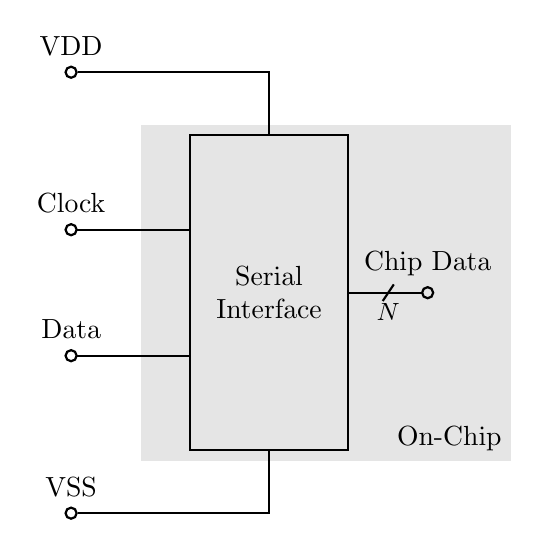
\begin{tikzpicture}
            [
                module/.style = {draw, rectangle, thick, minimum height = 4cm, minimum width = 2cm, align = center},
                wire/.style = {thick},
                port/.style = {thick, circle, inner sep = 0pt, minimum size = 4pt, draw = black, fill = white},
                bit line/.style = {
                    wire,
                    postaction = decorate,
                    decoration = {
                        markings,
                        mark = at position 0.5 with { \draw (-#1, {-1.5 * #1}) -- (#1, {1.5 * #1}); }
                    }
                },
                bit line/.default = 2pt,
                bitanno/.style = {font = \small}
            ]
            \node[module] (interface) {Serial\\Interface};
            \coordinate (leftfitboundary) at ($(interface.west)+(-0.5, 0.8)$);
            \draw[wire] ($(interface.west)+(0, 0.8)$) -- ++(-1.5, 0) node[port, label = above:Clock] (clock) {};
            \draw[wire] ($(interface.west)-(0, 0.8)$) -- ++(-1.5, 0) node[port, label = above:Data] (datain) {};
            \node[port, label = above:VDD] (vdd) at ($(clock)+(0,  2)$) {};
            \node[port, label = above:VSS] (vss) at ($(datain)+(0, -2)$) {};
            \draw[wire] (vdd) -| (interface.north);
            \draw[wire] (vss) -| (interface.south);
            \draw[bit line] (interface.east) -- node[below, bitanno] {$N$} ++(1, 0) node[port, label = {[name = chipdatalabel] above:Chip Data}] (chipdata) {};
            \node[fill = black, fill opacity = 0.1, fit = (interface) (leftfitboundary) (chipdata) (chipdatalabel)] (fit) {};
            \node[above left = 0cm] at (fit.south east) {On-Chip};
        \end{tikzpicture}
        \caption{Block Diagram of the Serial Interface}
        \label{fig:blockdiagram}
    \end{figure}
    
    The clock is always provided by the driver circuit (off-chip), the data are bidirectional.
    \section{Communication Protocol}
    The serial interface is state-based and command-driven.
    The following commands are supported and their bit patterns are documented in table~\ref{tab:commandpatterns}:
    \begin{itemize}
        \item \command{RESET}

            Reset the entire register to its default value.
            This only resets the main registers that face the circuits on the chip.
            The communication registers are not affected, which means that an update of the main registers following a reset does not necessarily
            ensure default data.
        \item \command{START\_SEND}

            Start the transmission of data from the driver to the chip.
            The data directly follow the command.
            The interface assumes that the correct number of bits is sent.
            It is not possible to send any number of bits different from the actual data length of the interface.
        \item \command{START\_RECEIVE}

            Start the reception of data from the chip to the driver.
            This is the only state where the chip drives the data line.
            Following this command, the driver must disable the output buffers that drive the data line, that is, enter a high-Z mode.
            This must happen in half of a clock cycle (see detailed timing diagram below).
            The interface then sends out the current $N$ bits that are stored in the interface.
            Only the data in the communication registers is sent, not what is actually stored in the main registers facing the circuits on the
            chip.
            It is not possible to read the data stored in the main registers.
        \item \command{UPDATE}

            Apply the data stored in the communication registers to the main registers.
            The data out of the interface (the bus that goes into the chip) only reflects this data.
            Without an update, this data is never changed.
            This ensures that there is no garbage data while the communication registers are being written.
            Usually an update directly follows a send command.
    \end{itemize}
    \begin{table}[htb]
        \centering
        \begin{tabular}{ll}
            \toprule
            Command                     & Pattern \\
            \midrule
            \command{RESET}             & \command{00} \\
            \command{START\_SEND}       & \command{01} \\
            \command{START\_RECEIVE}    & \command{01} \\
            \command{UPDATE}            & \command{01} \\
            \bottomrule
        \end{tabular}
        \caption{Bit Patterns of Commands}
        \label{tab:commandpatterns}
    \end{table}

    All commands are preceeded by a start sequence.
    The default (and currently implemented) sequence is \command{101}.

    \section{Implementation}
    \subsection{Register Cells}
    \subsubsection{Register Cell 0}
    \begin{tikzpicture}
        [
            every label/.style = {font = \ttfamily\scriptsize}
        ]
        \node[mux] (hold_write_mux) {};
        \node[dflipflop, right = of hold_write_mux.out, anchor = D] (dff_in) {};
        \node[dflipflop, circuits/dflipflop/negative clock edge = true, right = of dff_in] (dff_out) {};
        \node[mux, right = 1.5cm of dff_out.Q, anchor = in2] (dff_buf_mux) {};
        \node[andgate, right = of dff_buf_mux.out, anchor = in1] (reset_and_gate) {};
        \node[dflipflop, right = of reset_and_gate.out, anchor = D] (dff_buf) {};
        \node[dflipflop, circuits/dflipflop/negative clock edge = true, right = of dff_buf] (dff_store) {};
        % wires
        \draw[wire] (hold_write_mux.in2) -- ++(-1, 0) node[port, label=above:{Chain In}] {};
        \draw[wire] (hold_write_mux.botcontrol) |- ++(-1, -1) node[port, label=above:{enable}] (enableport) {};
        \draw[wire] (hold_write_mux.out) -- (dff_in.D);
        \draw[wire] (dff_out.Q) -- ++(0.5, 0) node[dot] (chain_out_dot) {} -- ++(0, 1) -| ($(hold_write_mux.in1)+(-0.5, 0)$) -- (hold_write_mux.in1);
        \draw[wire] (chain_out_dot) -- (dff_buf_mux.in2);
        \draw[wire] (dff_buf_mux.out) -- (reset_and_gate.in1);
        \draw[wire] (dff_in.Q) -- (dff_out.D);
        \draw[wire] (reset_and_gate.out) -- (dff_buf.D);
        \draw[wire] (dff_buf.Q) -- node[dot] (bit_out) {} (dff_store.D);
        \draw[wire] (dff_store.Q) -- ++(0.5, 0) -- ++(0, 1) -| ($(dff_buf_mux.in1)+(-0.5, 0)$) -- (dff_buf_mux.in1);
        \draw[wire] (dff_buf_mux.botcontrol) |- ++(-1, -1) node[port, label=above:{update}] (updateport) {};
        \draw[wire] (reset_and_gate.in2) -- ++(-0.5, 0) |- ++(-0.5, -1) node[port, label=above:{reset}] (resetport) {};
        \draw[wire] (bit_out) -- ++(0, 2) node[port, label=above:{Bit Out}] (bitoutport) {};
        % clk
        \node[port, below = of enableport, label = above:clk] (clkport) {};
        \draw[wire] (clkport) -| node[dot] (clk1) {} ($(dff_in.CLK)+(-0.5, 0)$) -- (dff_in.CLK);
        \draw[wire] (clk1) -| node[dot] (clk2) {} ($(dff_out.CLK)+(-0.5, 0)$) -- (dff_out.CLK);
        \draw[wire] (clk2) -| node[dot] (clk3) {} ($(dff_buf.CLK)+(-0.5, 0)$) -- (dff_buf.CLK);
        \draw[wire] (clk3) -| ($(dff_store.CLK)+(-0.5, 0)$) -- (dff_store.CLK);
    \end{tikzpicture}
    \subsubsection{Register Cell 1}
    \begin{tikzpicture}
        [
            every label/.style = {font = \ttfamily\scriptsize}
        ]
        \node[mux] (hold_write_mux) {};
        \node[dflipflop, right = of hold_write_mux.out, anchor = D] (dff_in) {};
        \node[dflipflop, circuits/dflipflop/negative clock edge = true, right = of dff_in] (dff_out) {};
        \node[mux, right = 1.5cm of dff_out.Q, anchor = in2] (dff_buf_mux) {};
        \node[notgate, right = of dff_buf_mux.out, anchor = in] (update_store_not_gate) {};
        \node[nandgate, right = of update_store_not_gate.out, anchor = in1] (reset_and_gate) {};
        \node[dflipflop, right = of reset_and_gate.out, anchor = D] (dff_buf) {};
        \node[dflipflop, circuits/dflipflop/negative clock edge = true, right = of dff_buf] (dff_store) {};
        % wires
        \draw[wire] (hold_write_mux.in2) -- ++(-1, 0) node[port, label=above:{Chain In}] {};
        \draw[wire] (hold_write_mux.botcontrol) |- ++(-1, -1) node[port, label=above:{enable}] (enableport) {};
        \draw[wire] (hold_write_mux.out) -- (dff_in.D);
        \draw[wire] (dff_out.Q) -- ++(0.5, 0) node[dot] (chain_out_dot) {} -- ++(0, 1) -| ($(hold_write_mux.in1)+(-0.5, 0)$) -- (hold_write_mux.in1);
        \draw[wire] (chain_out_dot) -- (dff_buf_mux.in2);
        \draw[wire] (dff_buf_mux.out) -- (update_store_not_gate.in);
        \draw[wire] (update_store_not_gate.out) -- (reset_and_gate.in1);
        \draw[wire] (dff_in.Q) -- (dff_out.D);
        \draw[wire] (reset_and_gate.out) -- (dff_buf.D);
        \draw[wire] (dff_buf.Q) -- node[dot] (bit_out) {} (dff_store.D);
        \draw[wire] (dff_store.Q) -- ++(0.5, 0) -- ++(0, 1) -| ($(dff_buf_mux.in1)+(-0.5, 0)$) -- (dff_buf_mux.in1);
        \draw[wire] (dff_buf_mux.botcontrol) |- ++(-1, -1) node[port, label=above:{update}] (updateport) {};
        \draw[wire] (reset_and_gate.in2) -- ++(-0.5, 0) |- ++(-0.5, -1) node[port, label=above:{reset}] (resetport) {};
        \draw[wire] (bit_out) -- ++(0, 2) node[port, label=above:{Bit Out}] (bitoutport) {};
        % clk
        \node[port, below = of enableport, label = above:clk] (clkport) {};
        \draw[wire] (clkport) -| node[dot] (clk1) {} ($(dff_in.CLK)+(-0.5, 0)$) -- (dff_in.CLK);
        \draw[wire] (clk1) -| node[dot] (clk2) {} ($(dff_out.CLK)+(-0.5, 0)$) -- (dff_out.CLK);
        \draw[wire] (clk2) -| node[dot] (clk3) {} ($(dff_buf.CLK)+(-0.5, 0)$) -- (dff_buf.CLK);
        \draw[wire] (clk3) -| ($(dff_store.CLK)+(-0.5, 0)$) -- (dff_store.CLK);
    \end{tikzpicture}
\end{document}

